
%%%%%%%%%%%%%%%%%%%%%%% file typeinst.tex %%%%%%%%%%%%%%%%%%%%%%%%%
%
% This is the LaTeX source for the instructions to authors using
% the LaTeX document class 'llncs.cls' for contributions to
% the Lecture Notes in Computer Sciences series.
% http://www.springer.com/lncs       Springer Heidelberg 2006/05/04
%
% It may be used as a template for your own input - copy it
% to a new file with a new name and use it as the basis
% for your article.
%
% NB: the document class 'llncs' has its own and detailed documentation, see
% ftp://ftp.springer.de/data/pubftp/pub/tex/latex/llncs/latex2e/llncsdoc.pdf
%
%%%%%%%%%%%%%%%%%%%%%%%%%%%%%%%%%%%%%%%%%%%%%%%%%%%%%%%%%%%%%%%%%%%


\documentclass[runningheads,a4paper]{llncs}

\usepackage{amssymb}
\setcounter{tocdepth}{3}
\usepackage{graphicx}
%\usepackage{natbib}
\usepackage{tikz}
%\usepackage{hyperref}
\usetikzlibrary{arrows}
\usepackage{fancyeq}

\newcommand{\citep}[1]{\cite{#1}}
\newcommand{\citet}[1]{\cite{#1}}

\usepackage{xcolor}
\newcommand{\todo}[1]{[{\color{blue}#1}]}

\usepackage{url}
\urldef{\mailsa}\path|{alfred.hofmann, ursula.barth, ingrid.haas, frank.holzwarth,|
\urldef{\mailsb}\path|anna.kramer, leonie.kunz, christine.reiss, nicole.sator,|
\urldef{\mailsc}\path|erika.siebert-cole, peter.strasser, lncs}@springer.com|    
\newcommand{\keywords}[1]{\par\addvspace\baselineskip
\noindent\keywordname\enspace\ignorespaces#1}

\newcommand {\lbrac} {\makebox[0pt]{[\kern-1ex[}}
\newcommand {\rbrac} {\makebox[0pt]{]\kern-1ex]}}
\newcommand{\denote}[1]{\lbrac~#1~\rbrac}
\newcommand{\amnote}[1]{{\marginpar{\raggedright\footnotesize\color{red}{#1}}}}

\tikzstyle{int}=[draw, minimum size=2em]
\tikzstyle{init} = [pin edge={thin,gray}]

\begin{document}

\mainmatter  % start of an individual contribution

% first the title is needed
\title{A tale of two abstractions:\\Monad transformers and object-orientation}

% Monads: the world's finest object-oriented programming language
% Exploring object-oriented programming with monads
% Functional programming: the world's finest object-oriented programming language

% a short form should be given in case it is too long for the running head
%\titlerunning{Programming with monadic state hierarchies}

% the name(s) of the author(s) follow(s) next
%
% NB: Chinese authors should write their first names(s) in front of
% their surnames. This ensures that the names appear correctly in
% the running heads and the author index.
%
\author{Michael B. Gale \and Alan Mycroft}
%
%\authorrunning{Lecture Notes in Computer Science: Authors' Instructions}
% (feature abused for this document to repeat the title also on left hand pages)

% the affiliations are given next; don't give your e-mail address
% unless you accept that it will be published
\institute{Computer Laboratory, University of Cambridge}

%
% NB: a more complex sample for affiliations and the mapping to the
% corresponding authors can be found in the file "llncs.dem"
% (search for the string "\mainmatter" where a contribution starts).
% "llncs.dem" accompanies the document class "llncs.cls".
%

\toctitle{Lecture Notes in Computer Science}
\tocauthor{Authors' Instructions}
\maketitle


\begin{abstract}
%We present an encoding of the principal features of object-oriented languages in pure Haskell. Our system supports object classes, inheritance, subtype polymorphism, dynamic dispatch, and open recursion. We establish a correspondence between inheritance and monad transformers by defining a state monad transformer for each class, parametrised only over the class's own state. The methods of a class are monadic computations which run on top of a stack of monad transformers, consisting of one layer for the class and each of its ancestors. Well-known limitations of monad transformers are overcome by the dynamic dispatch mechanism. The encoding allows class hierarchies to be open for extension in separately-compiled modules, therefore allowing the construction of modular programs. We show how to translate to our encoding from a small object-oriented language. Finally, we provide a Template Haskell implementation of this translation.

%Monad transformers are infamous for being awkward to work with. By only considering state monad transformers, we show that there exists a correspondence to the usual inheritance mechanism of object-oriented languages. While such languages take care of the boilerplate required for inheritance to work seamlessly, this is not the case for monad transformers. We exploit this correspondence and combine state monad transformers with the principal features of object-oriented languages, allowing us to treat stacks of state monad transformers like objects. We illustrate using examples that these objects are as easy to work with as their counterparts in object-oriented languages. Additionally, if we extend our system with an encoding for subtyping, we are able to write modular programs. Our system is encoded entirely in Haskell and requires no new language features. A Template Haskell library allows programmers to write class definitions in the same style as in object-oriented languages which then get translated to the corresponding encodings. We hope that our findings will form the foundation for a generalised system in which classes can have effects other than state.


Monad transformers are infamous for being awkward to work with. To begin tackling this problem, we formulate a correspondence between state monad transformers and the inheritance mechanism of object-oriented languages. While object-oriented languages implicitly supply the boilerplate required for inheritance to work seamlessly, state monad transformers require it to be explicit. By hiding this boilerplate in type class instances, we gain the ease of member access of object-oriented languages. This allows us to use stacks of state monad transformers as easily as objects. We illustrate using examples that these `objects' are as easy to work with as their object-oriented counterparts.

Our `object classes' do not need to know about other `object classes' which inherit from them. The resulting hierarchy is therefore open for extension. This can be taken advantage of to construct modular data types and programs through the addition of an encoding for subtyping as well as inheritance. All of this is encoded entirely in Haskell and requires no new language features. Finally, a Template Haskell library allows programmers to write class definitions in the same style as in object-oriented languages and in which the boilerplate is automatically derived.



%This opens up an exciting new 
%By establishing the effect of monad transformers to be a generalised form of inheritance, we show that state monad transformers can be used as natural interpreters for an object-oriented language. 

 

\keywords{Haskell, Monad Transformers, Object-Oriented Programming}
\end{abstract}

\section{Introduction}
\label{sec:introduction}

In a purely-functional programming language, such as Haskell, we might wish to write an application which interacts with an in-memory database. Since values are immutable, an update to the database returns a new, updated copy of it. To avoid having to keep track of the most recent version of the database, we use the state monad:
\begin{displaymath}
\begin{array}{lcl}
\multicolumn{3}{l}{\mathbf{type}~\mathit{MyDatabase} = \mathit{State}~\mathit{SqlDatabase}}\\
\mathit{runQuery} & :: & \mathit{String} \to \mathit{MyDatabase}~\mathit{SqlReader}
\end{array}
\end{displaymath}
The database is represented by the $\mathit{SqlDatabase}$ type and is used as an argument to the $\mathit{State}$ type, which represents the state monad. For convenience, we define $\mathit{MyDatabase}$ an alias for this. The type of $\mathit{runQuery}$ tells us that, if given an SQL query represented as a string of characters, it will run the query using an underlying database and give us back a result, represented by the $\mathit{SqlReader}$ type. The implementation of this function is not important, but note that its codomain is $\mathit{MyDatabase}~\mathit{SqlReader}$, meaning that the result is returned with the effect of mutating a database. 

Writing an application using just $\mathit{runQuery}$ may be prone to errors, however. For example, if the name of a table or column changes, all queries which refer to it must be updated as well. A common solution for this is to abstract over the entity model of the database, instead of writing SQL queries directly. For this purpose, we define a data type which represents our entity model. In this example, we have a table containing recipes, indexed by a unique, numeric identifier:
\begin{displaymath}
\begin{array}{lcl}
\multicolumn{3}{l}{\mathbf{data}~\mathit{Model} = \mathit{MkModel}~(\mathit{Map}~\mathit{Int}~\mathit{Recipe})}
\end{array}
\end{displaymath}
The model caches all changes we make to the table and only updates the database when we wish to do so. To implement this, we layer the model on top of the database using the state monad transformer $\mathit{StateT}$, creating a \emph{monad stack} in the process:
\begin{displaymath}
\begin{array}{lcl}
\multicolumn{3}{l}{\mathbf{type}~\mathit{DbModel} = \mathit{StateT}~\mathit{Model}~\mathit{MyDatabase}}\\\\
\mathit{saveChanges} & :: & \mathit{DbModel}~() \\
\mathit{saveChanges} & = & \mathbf{do} \\
\multicolumn{3}{l}{\qquad \begin{array}{lcl}
    m & \leftarrow & \mathit{get} \\
    \multicolumn{3}{l}{\mathbf{let}} \\
    \multicolumn{3}{l}{\qquad \mathit{query} = \ldots} \\
    \multicolumn{3}{l}{\mathit{lift}~(\mathit{runQuery}~\mathit{query})}\\
    \multicolumn{3}{l}{\mathit{return}~()}
\end{array} }
\end{array}
\end{displaymath}
The $\mathit{saveChanges}$ function is responsible for updating the database according to the cached changes. Firstly, it obtains the current state of the model $m$. It then generates a corresponding query, but this process is not important here so that it has been omitted. Lastly, the function calls $\mathit{runQuery}$ with the generated query. Note, however, that we must wrap the call to $\mathit{runQuery}$ in a call to $\mathit{lift}$ since $\mathit{runQuery}$ cannot run directly on the extended monad stack. Let us note here that putting two state monads on top of each other is isomorphic to having a single state monad with a pair combining the states. However, we believe that the latter approach makes code less reusable since the $\mathit{runQuery}$ function would be entirely incompatible with the new monad stack and would have to be rewritten. By putting another state monad on top, the old definition can be reused.

To use this implementation, we must also write the following:
\begin{displaymath}
\begin{array}{l}
\mathit{runState}~(\mathit{runStateT}~\mathit{go}~\mathit{emptyModel})~\mathit{initialDatabase} \\
\qquad \mathbf{where} \\
\qquad \qquad \begin{array}{lcl}
\mathit{go} & = & \mathbf{do} \\
\multicolumn{3}{l}{\qquad \begin{array}{l}
\mathtt{\{-~do~work~-\}}\\
\mathit{saveChanges}
\end{array}} 
\end{array}
\end{array}
\end{displaymath}
One way of interpreting the $\mathit{runState}$ and $\mathit{runStateT}$ functions is as the equivalent of opening a new scope in a language like C, which causes additional variables to be stored on the stack. The calls to $\mathit{lift}$ correspond to following indirections on the stack to locate variables. Another way of viewing this behaviour is as inheritance as we know it from object-oriented programming: the outer state monad transformer has access to the inner state monad transformer's state, thus effectively inheriting it. $\mathit{lift}$ is like an explicit $\mathit{super}$ in Java or $\mathit{base}$ in C\#. Writing $\mathit{lift}~(\mathit{runQuery}~\mathit{query})$ is equivalent to writing $\mathit{this}.\mathit{super}.\mathit{runQuery}(\mathit{query})$ in pseudo Java. Equally, writing $\mathit{runState}~f~\mathit{db}$ is the equivalent of $\mathit{db}.\mathit{f}$ in Java.

Neither interpretation requires the programmer to explicitly implement the respective behaviour in other languages, yet it has to be made explicit for monad transformers in Haskell. We believe that this is at least partially due to the lack of names in monad stacks, while local variables in C and class members in object-oriented languages both have names. In Haskell's \texttt{mtl} library, type classes are used to allow for the automatic lifting of functions such as $\mathit{get}$ and $\mathit{put}$ through a monad stack, if there is only one state monad in it. In other words, it addresses the naming problem for distinct effects, but not for several instances of the same effect.

Interestingly, if we add names to the computations which can be run on a monad stack, then it exposes a choice in programming styles commonly known as the expression problem\cite{wadler1998expression}. Without names, we can add both layers and computations to a monad stack at will, but have to manually call the $\mathit{lift}$ function. With names, we can automatically generate calls to $\mathit{lift}$, but computations can no longer be added at will.

In this work, we treat stacks of state monad transformers as objects and allow programmers to define classes of state monad transformer stacks, thus limiting the set of computations which may be run, but avoiding the need for explicit $\mathit{lift}$ and $\mathit{runState}$ calls. Specifically, our contributions are:
\begin{itemize}
    \item We have established a relationship between inheritance and (state) monad transformers, allowing us to exploit well-known techniques in object-oriented programming for monadic programming. This relationship also leads to similarities to the expression problem, suggesting that we may have to choose between one advantage or the other.
    \item State monad transformers have had this behaviour all along, but thus far it has been awkward for programmers to make use of it. We show how to encode a simple object system in Haskell which exploits the correspondence to inheritance in order to simplify the usage of state monads (Section 2).
    \item By adding an encoding of subtyping to our system which represents objects as functional zippers, we enable a third type of polymorphism within Haskell. If we have an object class $B$ which is a subtype of an object class $A$, then there is a representation of a $B$ object which has type $A$. As a result, subtype polymorphism also enables programmers to construct modular data types. Our approach does not require whole-program compilation unlike, for example, open data types and functions \cite{loh2006open} (Section 3).
    \item We use Template Haskell to provide a convenient method for programmers to generate such encodings from class definitions without any new extensions to the host language. We require no transformation of any function or method definitions as our library implements the combinators in standard Haskell (Section 4).
\end{itemize}

\textbf{-- OLD INTRODUCTION --}

Different programming paradigms evolve independently, but occasionally cross-pollination takes place. Features characteristic of the functional paradigm, such as \emph{e.g.} anonymous and higher-order functions, have made their way into object-oriented languages such as \emph{e.g.} C\# and Java 8. Often this cross-pollination highlights other issues. For example, immutability is useful for functional constructs but hard to express in Java. Similarly, work combining functional and logic programming \citep{nadathur1988overview,hanus2006curry,somogyi1996execution} helped us better understand interactions of backtracking and laziness, and higher-order functions and unification.

In this work, we encode object-oriented features in a purely functional language, namely Haskell. Doing so not only allows programmers to explore new ways of structuring functional programs, but also casts light in the opposite direction---adding a new point in the old object-oriented debate concerning the difference between subtyping and inheritance \cite{cook1989inheritance}. 

For convenience, we present syntactic sugar for our object system on top of standard Haskell. This de-sugars back to pure Haskell and monads in a way entirely
parallel to the way that Haskell's $\mathbf{do}$-notation does for imperative code.

Object-oriented programming as a paradigm describes a range of related concepts in the same way that functional programming does. However, languages which associate themselves with one paradigm rarely support all of its characteristic features. \citet{armstrong2006quarks}, for example, surveys object-oriented languages in an attempt to identify what concepts characterise object-oriented programming. According to Armstrong, some of the most common features in such languages are: dynamic dispatch, encapsulation, subtype polymorphism, and inheritance. 

It is already folklore that dynamic dispatch can be implemented in Haskell with existential types and type classes. In the following example, a value of type $\mathit{Bird}$ is constructed by applying the $\mathit{MkBird}$ constructor to some type $a$ for which there is an instance of the $\mathit{BirdLike}$ type class:
\begin{displaymath}
\begin{array}{lcl}
\mathbf{data}~\mathit{Bird} & = & \forall a. \mathit{BirdLike}~a \Rightarrow \mathit{MkBird}~a
\end{array}
\end{displaymath}
The $\mathit{Bird}$ type effectively serves as an abstract base class. It is not possible to obtain a value of this type without some other type $a$ which implements $\mathit{BirdLike}$. Any such type can be seen as a subtype of $\mathit{Bird}$ and type-casts to the base class are possible by applying the $\mathit{MkBird}$ constructor. The type class constraint ensures that every subtype has the properties we would expect of, in this example, a bird.

This is an intriguing concept, but is often perceived as an anti-pattern. After all, why should we bother with a base class type if we can simply place a type class constraint on every function expecting bird-like arguments and avoid the $\mathit{Bird}$ type all-together?

We answer this question and show how the above concept can be elevated from a neat trick without much practical use to the foundation of an object system for purely-functional languages with a range of benefits. Specifically, our contributions are:
\begin{itemize}
    \item We build upon the technique of using existential types combined with type classes to encode a comprehensive object system in Haskell, supporting object classes, inheritance, coercive subtype polymorphism, and non-aliased mutation. In Section \ref{sec:usage} we first show how objects in our encoding are used within a standard Haskell program, before describing the encoding itself in Section \ref{sec:encoding}.
    \item Class hierarchies in our encoding are open for extension and do not require whole-program compilation. We thereby improve upon approaches which do, such as \emph{e.g.} open data types and functions \cite{loh2006open}.
    \item Our system enables open recursion, allowing methods of one object class to call other methods which have either no implementation (\emph{i.e.} are abstract) or are overriden by a deriving class.
    %\item Monad transformers \cite{moggi1989abstract,jones1995transformers} allow monadic effects to be layered on top of each other to form ``monad stacks''. Functions which make use of the effects in this stack cannot always be called directly, however. If a function's effect does not match that of the whole stack, programmers must indicate explicitly how many layers would have to be taken off in order for it to match. In Haskell, this is accomplished by wrapping a function in a call to $\mathit{lift}$ for every monad in a stack of monad transformers that should be skipped. Our system hides this boilerplate in the dynamic dispatch mechanism. 
    \item We show how to translate from a simple notation for object classes, following the conventions of object-oriented languages, to the corresponding encodings in Haskell (Section \ref{sec:auto}).
    \item This translation is implemented as a Haskell library using Template Haskell combined with a suitable set of combinators (Section \ref{sec:th}).
\end{itemize}

\textbf{-- END OF OLD INTRODUCTION --}
\section{Monad stacks and object-orientation}
\label{sec:objects}

Consider the database example from Section 1. As the programmer, we know when writing the $\mathit{saveChanges}$ function that $\mathit{runQuery}$ can be run on a smaller part of our monad stack. \emph{I.e.} it requires the monad stack to be $\mathit{State}~\mathit{SqlDatabase}$, while the monad stack of $\mathit{saveChanges}$ also provides additional state on top of that. As a result of this type incompatibility, we must use $\mathit{lift}$ to wrap, in this case, the $\mathit{runQuery}$ function up in the type that corresponds to the one expected by $\mathit{saveChanges}$. If this layer is several levels away from the top of the stack, several, successive calls to $\mathit{lift}$ are required.

Let us refer to function calls which can be run on top of the monad stack -- \emph{i.e.} those functions which can directly be composed using $\bind$, with or without the help of $\mathit{lift}$ -- as \emph{internal calls} as opposed to \emph{external calls} which must be wrapped into calls to $\mathit{runX}$ functions, such as \emph{e.g.} $\mathit{runStateT}$, first. We will address internal calls first, before moving on to external calls later in this section. 

\subsection{Internal calls}

Most monadic computations in Haskell are represented by values of some data type, which can be combined with $\bind$ and ultimately evaluated by some corresponding $\mathit{runX}$ function. Monad transformers are therefore the data types belonging to monads, which are parametrised over and defined in terms of the data type belonging to some arbitrary monad. A monadic computation, such as $\mathit{runQuery}$ returns a value of the data type corresponding to the monad stack it runs on. Since $\mathit{runQuery}$ and $\mathit{saveChanges}$ run on top of different monad stacks, they return values of different, incompatible types. In order to use $\mathit{runQuery}$ on top of the same monad stack as $\mathit{saveChanges}$, it must return a value of the same type, because otherwise it cannot be composed using $\bind$ with other computations in the sequence. 

In other words, we really want $\mathit{runQuery}$ to be an overloaded function which returns a value of the monadic data type corresponding to the other computations in the same sequence. Overloading in Haskell is achieved through type classes, so instead of defining $\mathit{runQuery}$ as a global function with a specific type, we should instead define it as part of a type class:
\begin{displaymath}
\begin{array}{l}
\mathbf{class}~\mathit{SqlDatabaseCtx}~m~\mathbf{where}\\
\qquad \begin{array}{lcl}
\mathit{runQuery} & :: & \mathit{String} \to m~\mathit{SqlReader}
\end{array}
\end{array}
\end{displaymath}
This type class has a single parameter $m$ which represents the context in which $\mathit{runQuery}$ should be callable. In other words, $m$ should be the data type which corresponds to a monad stack on top of which $\mathit{runQuery}$ can be run. To restore the old functionality, we must provide an instance for $\mathit{SqlDatabaseCtx}$ for the simplest monad stack on top of which $\mathit{runQuery}$ can be run\footnote{Note that this requires the \texttt{FlexibleInstances} language extension.}:
\begin{displaymath}
\begin{array}{l}
\mathbf{instance}~\mathit{SqlDatabaseCtx}~\mathit{MyDatabase}~\mathbf{where}\\
\qquad \begin{array}{lcl}
\mathit{runQuery}~\mathit{query} & = & \ldots
\end{array}
\end{array}
\end{displaymath}
We once again omit the exact definition of $\mathit{runQuery}$, but it remains unchanged from the previous implementation. In order to call $\mathit{runQuery}$ on the monad stack used by $\mathit{saveChanges}$, we need a second instance for this particular monad stack:
\begin{displaymath}
\begin{array}{l}
\mathbf{instance}~\mathit{SqlDatabaseCtx}~\mathit{DbModel}~\mathbf{where}\\
\qquad \begin{array}{lcl}
\mathit{runQuery}~\mathit{query} & = & \mathit{lift}~(\mathit{runQuery}~\mathit{query})
\end{array}
\end{array}
\end{displaymath}
This bears similarity to, for example, the type-theoretic account of object-oriented programming given by Pierce and Turner\cite{pierce1994simple}, where methods inherited from parental classes must also be adapted in a similar style. We can now rewrite the definition of $\mathit{saveChanges}$ to get rid of the explicit call to $\mathit{lift}$:
\begin{displaymath}
\begin{array}{lcl}
\mathit{saveChanges} & :: & \mathit{DbModel}~() \\
\mathit{saveChanges} & = & \mathbf{do} \\
\multicolumn{3}{l}{\qquad \begin{array}{lcl}
    m & \leftarrow & \mathit{get} \\
    \multicolumn{3}{l}{\mathbf{let}} \\
    \multicolumn{3}{l}{\qquad \mathit{query} = \ldots} \\
    \multicolumn{3}{l}{\mathit{runQuery}~\mathit{query}}\\
    \multicolumn{3}{l}{\mathit{return}~()}
\end{array} }
\end{array}
\end{displaymath}
Instead of having to write $\mathit{lift}~(\mathit{runQuery}~\mathit{query})$ every time we wish to use $\mathit{runQuery}$ in computations belonging to our entity model, we can just write $\mathit{runQuery}$ by itself. This saves us from having to write $\mathit{lift}$ every time $\mathit{runQuery}$ is used, at the cost of having to declare $\mathit{runQuery}$ as part of a type class and providing an implementation for every context in which we wish to use it. We must also know of all computations we wish to use in this style when we declare, in this case, the $\mathit{SqlDatabaseCtx}$ type class. Although, right now there is nothing that stops us from having several type classes per monad stack, we will not have this luxury later on, exposing the relationship to the expression problem.

\subsection{Monad stack configurations}
\label{sec:configurations}

Since monadic computations are just values of some data type, they cannot just be invoked like normal functions. Instead, each monad $X$ has a corresponding $\mathit{runX}$ function which can be used to evaluate a computation in the presence of its effect. If we have a stack of monads, then successive calls to these functions are required for each layer in the stack, as shown in Section 1. This is often cumbersome as the programmer has to remember to insert the calls to these $\mathit{runX}$ functions, place them in the right order, and supply them with the right arguments. Instead, we would much rather like to just supply the monadic computation with its initial configuration, such as the initial state of the state monad, in the same style that a method is invoked on an object. For example, instead of writing $\mathit{runState}~\mathit{foo}~\mathit{state}$, we want to write the equivalent of $\mathit{state}.\mathit{foo}$ and similarly for more complicated stacks of monads. This is what we refer to as \emph{external calls}, while an internal call is one that does not require a ``configuration'' to be supplied -- \emph{i.e.} the equivalent of a call that can optionally be prefixed by $\mathbf{this}$ in Java. 

Before we can show how to implement external calls, let us first introduce a notation of \emph{monad stack configurations} or, more simply, ``objects''. An object in our system is a value which describes the layers of a monad stack. Each layer is described by what we will call a $\Delta$-object. When an object is supplied as part of an external call, it provides all the required information for the callee to call the appropriate $\mathit{runX}$ functions and in the appropriate order, so that the monadic computation corresponding to the call can be evaluated. In other words, the function invoked for an external call is a wrapper around the monadic computation which traverses the $\Delta$-objects within an object. Once the monadic computation has been evaluated, the wrapper will return an updated object as well as a result to the caller. For this paper, we will only consider $\Delta$-objects corresponding to state monads, although in principle nothing prohibits us from constructing $\Delta$-objects which correspond to other monads.

Objects and $\Delta$-objects are represented using algebraic data types. In the case of the bottom layer of a monad stack, there is only a single $\Delta$-object which makes up the object. We assume that there exists some specification for the structure of the monad stack which we shall refer to as \emph{object classes}. An object class can either be a \emph{base class}, representing the bottom of a monad stack, or a \emph{sub-class}, representing an extension to some other monad stack. For state monads and this paper, we may think of them as the same as Java classes. Each class contains a set of fields, representing the state of the corresponding state monad, as well as a set of methods, representing the monadic computations which are part of a corresponding type class and can automatically be $\mathit{lift}$ed. 

The type of $\Delta$-objects for an object class describing the $\mathit{MyDatabase}$ monad from our running example can be defined as follows:
\begin{displaymath}
\begin{array}{lcl}
\mathbf{data}~\mathit{MyDatabaseObj} & = & \mathit{MkMyDatabaseData}~\{ \\
\multicolumn{3}{l}{\qquad \mathit{myDatabaseState} :: \mathit{SqlDatabase} }  \\
\} && 
\end{array}
\end{displaymath}
Perhaps surprisingly, the object only stores the initial state of the monad stack represented by $\mathit{MyDatabase}$, namely $\mathit{State}~\mathit{SqlDatabase}$, but no indication that this $\Delta$-object represents a state monad layer in the stack. This is left to the wrapper function we will implement for the external call and is discussed in the following section. Since there is a 1:1 relationship between a $\Delta$-object and the corresponding type class, we can hard-code a $\mathit{runStateT}$ call for its instances.

For $\mathit{DbModel}$, the type of corresponding $\Delta$-objects looks as shown below:
\begin{displaymath}
\begin{array}{lcl}
\mathbf{data}~\mathit{DbModelObj} & = & \mathit{MkDbModelData}~\{ \\
\multicolumn{3}{l}{\qquad \begin{array}{lcl}
\mathit{dbModelParent} & :: & \mathit{MyDatabaseObj}, \\
\mathit{dbModelState} & :: & \mathit{Map}~\mathit{Int}~\mathit{Recipe}
\end{array}  }  \\
\} && 
\end{array}
\end{displaymath}
In addition to the state monad's initial state, we also store a $\Delta$-object belonging to the parental layer in the monad stack. Unlike in most object-oriented languages, where the inherited state is merged into a sub-class's state, we keep them separate. The reasoning for this is twofold: firstly, it saves us from having to copy and paste code, but secondly, and more importantly, the states need to be separate when the calls to $\mathit{runStateT}$ are made. The configuration required to call $\mathit{saveChanges}$ from our example can now be constructed as follows:
\begin{displaymath}
\mathit{config} = \mathit{MkDbModelData}~\mathit{emptyModel}~(\mathit{MkMyDatabaseData}~\mathit{initialDatabase})
\end{displaymath}
Importantly, instead of having two separate values for the monad stack's state, we have combined them into one configuration, although they are still separate within this configuration. The wrapper for an external call can traverse such a configuration to set up the monad stack layer-by-layer as we detail in the next section.

\subsection{External calls}

Every computation that is part of an object class can be called internally or externally. In this section, we show how to implement the wrapper functions for the external calls. For now, we use distinct names for the internal and external versions of a computation. However, we show how both can share the same name in Section \ref{sec:th}. 

To begin, we need to change how the type classes which represent the interfaces of our object classes are constructed. For $\mathit{SqlDatabase}$ we now have:
\begin{displaymath}
\begin{array}{l}
\mathbf{class}~\mathit{SqlDatabaseCtx}~\mathit{obj}~\mathit{st}~m \mid \mathit{obj} \to \mathit{st}, \mathit{st} \to \mathit{obj}~\mathbf{where}\\
\qquad \begin{array}{lcl}
\mathit{\_\mathit{sqlDatabaseCtx\_invoke}} & :: & \\
\multicolumn{3}{l}{\qquad \mathit{SqlDatabaseCtx}~\mathit{obj}'~\mathit{st}'~(\mathit{StateT}~\mathit{st}~\mathit{m}) \Rightarrow}\\
\multicolumn{3}{l}{\qquad \mathit{obj}' \to (\mathit{obj}' \to \mathit{StateT}~\mathit{st}~m~(r,\mathit{obj}')) \to} \\
\multicolumn{3}{l}{\qquad \mathit{obj} \to m~(r,\mathit{obj},\mathit{obj}')} \\\\
\mathit{\_int\_runQuery} & :: & \mathit{String} \to \mathit{StateT}~\mathit{st}~m~\mathit{SqlReader} \\
\mathit{\_ext\_runQuery} & :: & \mathit{obj} \to \mathit{String} \to m~(\mathit{SqlReader}, \mathit{obj})
\end{array}
\end{array}
\end{displaymath}
While we previously had a single-parameter type class whose parameter represented the type corresponding to a monad stack, we now have a multi-parameter type class with three parameters: $\mathit{obj}$ represents the type of an object which describes a monad stack capable of supporting the computations in the interface, $\mathit{st}$ which represents the state added by the object class of $\mathit{obj}$, and $m$ which represents the type of the parental context in which we wish to call the methods -- more on this later. 

We use functional dependencies\cite{jones2000type} to indicate that the object and state type uniquely determine each other. Therefore, only one needs to be known during type inference, in order to select an instance of the type class, even if it is not clear from a context what the type of the other parameter is.

The type class contains three methods: $\mathit{\_sqlDatabaseCtx\_invoke}$ which we will discuss later, and the internal and external versions of $\mathit{runQuery}$. Note that the type of the internal version of $\mathit{runQuery}$, with prefix $\_\mathit{int}\_$\footnote{As a convention, we will always use names starting with $\_$ to indicate definitions which are only meant to be used internally by our encoding.}, has changed as a result. Instead of $m~\mathit{SqlReader}$ where $m$ is the type corresponding to the full monad stack, we now assemble the type of the top layer in the method's type. This is necessary, because we must refer to the same $m$ in the type of $\mathit{runQuery\_ext}$. The type class instance(s) belonging to a $\Delta$-object can only call the $\mathit{runX}$ function for the layer in the monad stack which they represent and must therefore already be invoked from a context where the $\mathit{runX}$ functions for the monad stack up to that point have been invoked. To illustrate this procedure, the updated instance belonging to the $\mathit{MyDatabase}$ layer in our example is now:
\begin{displaymath}
\begin{array}{l}
\mathbf{instance}~\mathit{SqlDatabaseCtx}~\mathit{MyDatabaseObj}~\mathit{SqlDatabase}~\mathit{Identity}~\mathbf{where}\\
\qquad \begin{array}{lcl}
\mathit{\_\mathit{sqlDatabaseCtx\_invoke}}~\mathit{obj}~f~(\mathit{MkMyDatabaseData}~d) & = & \mathbf{do}\\
\multicolumn{3}{l}{\qquad \begin{array}{lcl}
((r, \mathit{obj'}, d')) & \leftarrow & \mathit{runStateT}~(f~\mathit{obj})~d \\
\multicolumn{3}{l}{\mathit{return}~(r, \mathit{MkMyDatabaseData}~d'), \mathit{obj}'}
\end{array}}
\\\\
\mathit{\_int\_runQuery}~\mathit{query} & = & ~\ldots \\
\mathit{\_ext\_runQuery}~(\mathit{MkMyDatabaseData}~\mathit{d})~v & = & \mathbf{do} \\
\multicolumn{3}{l}{\qquad (r,d') \leftarrow \mathit{runStateT}~(\mathit{\_int\_runQuery}~v)~d } \\ 
\multicolumn{3}{l}{\qquad \mathit{return}~(r, (\mathit{MkMyDatabaseData}~d')) } 
\end{array}
\end{array}
\end{displaymath}
The implementation of $\mathit{runQuery}$ still remains unchanged and is omitted for brevity, but is given the name $\mathit{\_int\_runQuery}$ here. Additionally, we now have the $\mathit{\_ext\_runQuery}$ method which inspects an object of type $\mathit{MyDatabaseObj}$, extracts the state, and uses it as the initial state for an invocation of $\mathit{runStateT}$. In this case, the $\mathit{MkMyDatabaseData}$ constructor represents an instance of a $\mathit{MyDatabaseObj}$ object and the computation evaluated by $\mathit{runStateT}$ is therefore the actual implementation of the $\mathit{runQuery}$ function. Finally, $\mathit{\_ext\_runQuery}$ returns the result obtained from the computation and wraps the state back up in an $\mathit{MyDatabaseObj}$ object.

In order to call the $\mathit{runX}$ functions in the order dictated by the class hierarchy, we must start from the base class, which represents the bottom of the monad stack, and work our way to the top. However, if we make an external call to a sub-class object, then it is handled by a type class instance for that sub-class object. That instance only knows how to invoke the $\mathit{runX}$ function for the layer in the monad stack corresponding to itself, and not those for its parents. If we were to try and set up the monad stack in a different order than the one given by the class hierarchy, then none of our definitions would work. The $\_\mathit{sqlDatabaseCtx\_invoke}$ function solves this problem, by providing a way for $\mathit{DbModel}$ objects and objects belonging to other sub-classes of $\mathit{MyDatabase}$ to request that the $\mathit{runX}$ function corresponding to the $\mathit{MyDatabase}$ layer should be invoked and an arbitrary computation, provided as argument to the $\_\mathit{invoke}$ function, should be evaluated.  One such $\_\mathit{invoke}$ function is added to every type class describing the interface of a layer in a monad stack. The process by which it works is illustrated in Figure \ref{fig:invoke}. 

All sub-classes have two instances of every type class they have to implement: one where $m$ is the type of the parental monad stack and one where $m$ is set to $\mathit{Identity}$. When an external call is made to a sub-class object, the instance of the appropriate type class where $m = \mathit{Identity}$ is selected. The implementation of the external version of a computation in this instance, such as $\_\mathit{ext}\_\mathit{saveChanges}$ in Figure \ref{fig:invoke}, forwards the call to its parent using the respective $\_\mathit{invoke}$ function. This continues until the base class is reached, whose only type class instance is for $m = \mathit{Identity}$. From this point onwards, the process proceeds as we have seen before. The base class invokes the $\mathit{runX}$ function for the first layer and forwards the call to the next $\Delta$-object in line, from the bottom to the top using the primary type class instances for the $\Delta$-objects, where $m$ is the type of the respective parental monad stack. 

\begin{figure}
    \begin{center}
        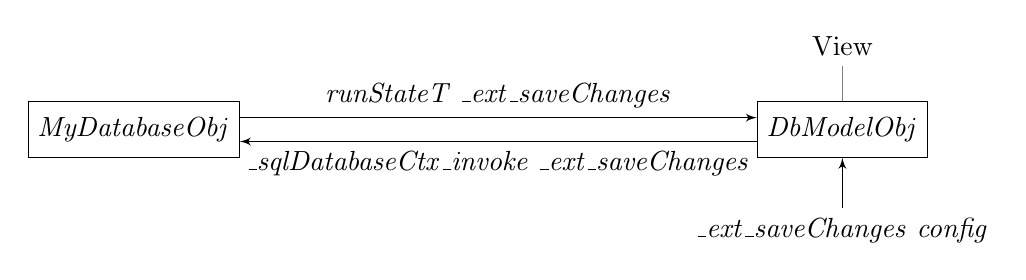
\begin{tikzpicture}[node distance=9.0cm,auto,>=latex']
        \node [int] (c)  {$\mathit{MyDatabaseObj}$};
        \node [int,pin={[init]above:View}] (d) [right of=c] {$\mathit{DbModelObj}$};
        \node (b) [below of=d,node distance=1cm, coordinate] {a};
        
        \path[->] ([yshift=1ex]c.east) edge node {$\mathit{runStateT~\_ext\_saveChanges}$} ([yshift=1ex]d.west);
        \path[->] ([yshift=-1ex]d.west) edge node {$\mathit{\_sqlDatabaseCtx}\_\mathit{invoke}~\mathit{\_ext\_saveChanges}$} ([yshift=-1ex]c.east);
        \path[->] (b.north) edge node [below, pos=-0] {$\mathit{\_ext\_saveChanges~config}$} (d.south);
        \end{tikzpicture} 
    \end{center}
    \caption{Invoking $\mathit{saveChanges}$ on an $\mathit{DbModelObj}$ object $\mathit{config}$} \label{fig:invoke}
\end{figure}

The $\mathit{DbModel}$ layer in our example has its own type class, for which $\mathit{SqlDatabaseCtx}$ is a super-class. This means that for every instance of $\mathit{DbModelCtx}$, there must also be an instance of $\mathit{SqlDatabaseCtx}$:
\begin{displaymath}
\begin{array}{l}
\mathbf{class}~\mathit{SqlDatabaseCtx}~\mathit{obj}~\mathit{st}~m \Rightarrow \\
\quad \mathit{DbModelCtx}~\mathit{obj}~\mathit{st}~m \mid \mathit{obj} \to \mathit{st}, \mathit{st} \to \mathit{obj}~\mathbf{where}\\\\
\qquad \begin{array}{lcl}
\mathit{\_\mathit{dbModelCtx\_invoke}} & :: & \\
\multicolumn{3}{l}{\qquad \mathit{DbModelCtx}~\mathit{obj}'~\mathit{st}'~(\mathit{StateT}~\mathit{st}~\mathit{m}) \Rightarrow}\\
\multicolumn{3}{l}{\qquad \mathit{obj}' \to (\mathit{obj}' \to \mathit{StateT}~\mathit{st}~m~(r,\mathit{obj}')) \to} \\
\multicolumn{3}{l}{\qquad \mathit{obj} \to m~(r,\mathit{obj},\mathit{obj}')} \\\\
\mathit{\_int\_saveChanges} & :: & \mathit{StateT}~\mathit{st}~m~\mathit{()} \\
\mathit{\_ext\_saveChanges} & :: & \mathit{obj} \to m~(\mathit{()}, \mathit{obj})
\end{array}
\end{array}
\end{displaymath}
As mentioned previously, there are two instances for every type class an object implements. The \emph{primary instance} for $\mathit{DbModelObj}$ where $m = \mathit{MyDatabase}$ is shown below. It follows exactly the same structure as the instance of $\mathit{SqlDatabaseCtx}$ for $\mathit{MyDatabaseObj}$:
\begin{displaymath}
\begin{array}{l}
\mathbf{instance}~\mathit{DbModelCtx}~\mathit{DbModelObj}~(\mathit{Map}~\mathit{Int}~\mathit{Recipe})~\mathit{MyDatabase}~\mathbf{where}\\\\
\qquad \begin{array}{lcl}
\mathit{\_\mathit{dbModelCtx\_invoke}} ~\mathit{obj}~f~(\mathit{MkMyDatabaseData}~d) & = & \mathbf{do}\\
\multicolumn{3}{l}{\qquad \begin{array}{lcl}
((r, \mathit{obj'}, d')) & \leftarrow & \mathit{runStateT}~(f~\mathit{obj})~d \\
\multicolumn{3}{l}{\mathit{return}~(r, \mathit{MkMyDatabaseData}~d'), \mathit{obj}'}
\end{array}}
\\\\
\multicolumn{3}{l}{\qquad \mathit{DbModelCtx}~\mathit{obj}'~\mathit{st}'~(\mathit{StateT}~\mathit{st}~\mathit{m}) \Rightarrow}\\
\multicolumn{3}{l}{\qquad \mathit{obj}' \to (\mathit{obj}' \to \mathit{StateT}~\mathit{st}~m~(r,\mathit{obj}')) \to} \\
\multicolumn{3}{l}{\qquad \mathit{obj} \to m~(r,\mathit{obj},\mathit{obj}')} \\\\
\mathit{\_int\_saveChanges} & = & \mathbf{do} \\
\multicolumn{3}{l}{\qquad \begin{array}{lcl}
    m & \leftarrow & \mathit{get} \\
    \multicolumn{3}{l}{\mathbf{let}} \\
    \multicolumn{3}{l}{\qquad \mathit{query} = \ldots} \\
    \multicolumn{3}{l}{\mathit{\_int\_runQuery}~\mathit{query}}\\
    \multicolumn{3}{l}{\mathit{return}~()}
\end{array} }\\
\mathit{\_ext\_saveChanges}~(\mathit{MkDbModelData}~p~d) & = & \mathbf{do} \\
\multicolumn{3}{l}{\qquad (r,d') \leftarrow \mathit{runStateT}~\mathit{\_int\_saveChanges}~d } \\ 
\multicolumn{3}{l}{\qquad \mathit{return}~(r, (\mathit{MkMyDatabaseData}~p~d')) } 
\end{array}
\end{array}
\end{displaymath}
The second instance of $\mathit{DbModelCtx}$ for $\mathit{DbModelObj}$, where $m = \mathit{Identity}$ is more interesting, since it implements the behaviour shown in Figure \ref{fig:invoke}.
% may need a lambda in the recursive invoke call

\begin{displaymath}
\begin{array}{l}
\mathbf{instance}~\mathit{DbModelCtx}~\mathit{DbModelObj}~(\mathit{Map}~\mathit{Int}~\mathit{Recipe})~\mathit{Identity}~\mathbf{where}\\
\qquad \begin{array}{lcl}
\mathit{\_\mathit{dbModelCtx\_invoke}}~\mathit{obj}~\mathit{f}~(\mathit{MkDbModelData}~p~d) & = & \mathbf{do} \\
\multicolumn{3}{l}{\qquad \mathit{(r,p',\mathit{MkDbModelData}~\_~d) \leftarrow}}\\
\multicolumn{3}{l}{\qquad \qquad \mathit{\_myDatabaseCtx\_invoke}~\mathit{obj}~\mathit{f}~p} \\
\multicolumn{3}{l}{\qquad \mathit{return}~(r,\mathit{MkDbModelData}~p'~d)} \\\\
\multicolumn{3}{l}{\qquad \mathit{obj}' \to (\mathit{obj}' \to \mathit{StateT}~\mathit{st}~m~(r,\mathit{obj}')) \to} \\
\multicolumn{3}{l}{\qquad \mathit{obj} \to m~(r,\mathit{obj},\mathit{obj}')} \\\\

\mathit{\_ext\_saveChanges}~\mathit{obj}@(\mathit{MkDbModelData}~p~\_) & = & \mathbf{do} \\
\multicolumn{3}{l}{\qquad (r,p',\mathit{MkDbModelData}~\_~d) \leftarrow} \\
\multicolumn{3}{l}{\qquad \qquad \mathit{\_myDatabaseCtx\_invoke}~\mathit{obj}~\mathit{\_ext\_saveChanges}~p} \\
\multicolumn{3}{l}{\qquad \mathit{return}~(r,\mathit{MkDbModelData}~p'~d)}
\end{array}
\end{array}
\end{displaymath}
\section{Subtyping}
\label{sec:encoding}

A pleasant property of class hierarchies in object-oriented languages is that they are open for extension. In other words, classes do not need to know about other classes which inherit from them. For example, consider the following, abstract base class for an expression language in Java:
\begin{displaymath}
\begin{array}{l}
\mathbf{abstract}~\mathbf{class}~\mathit{Expr}~\{\\
\qquad \mathbf{public}~\mathbf{abstract}~\mathit{int}~\mathit{eval}();\\
\}
\end{array}
\end{displaymath}
This roughly corresponds to an algebraic data type $\mathit{Expr}$ in Haskell with no constructors and a function $\mathit{eval} :: \mathit{Expr} \to \mathit{Int}$. However, while we cannot retrospectively add constructors to a data type in Haskell, we can extend the $\mathit{Expr}$ class in Java:
\begin{displaymath}
\begin{array}{l}
\mathbf{class}~\mathit{Val}~\mathbf{extends}~\mathit{Expr}~\{\\
\qquad \mathbf{private}~\mathit{int}~\mathit{value};\\\\
\qquad \mathbf{public}~\mathit{int}~\mathit{eval}()~\{\\
\qquad \qquad \mathbf{return}~\mathit{this}.\mathit{value};\\
\qquad \}\\
\}
\end{array}
\end{displaymath}
The author of the $\mathit{Expr}$ class does not need to know about the $\mathit{Val}$ class and may even compile a library only containing $\mathit{Expr}$. The class can still be extended in other libraries by other authors, however. Our object system from Section \ref{sec:objects} allows for the same, but it has one major limitation: there is no support for subtyping that would allow us to \emph{e.g.} cast a $\mathit{DbModel}$ object to a $\mathit{MyDatabase}$ object. To see why this is an important limitation, consider the following sub-class for $\mathit{Expr}$ in Java:
\begin{displaymath}
\begin{array}{l}
\mathbf{class}~\mathit{Add}~\mathbf{extends}~\mathit{Expr}~\{\\
\qquad \mathbf{private}~\mathit{Expr}~\mathit{left};\\
\qquad \mathbf{private}~\mathit{Expr}~\mathit{right};\\\\
\qquad \mathbf{public}~\mathit{int}~\mathit{eval}()~\{\\
\qquad \qquad \mathbf{return}~\mathit{this}.\mathit{left}.\mathit{eval}() + \mathit{this}.\mathit{right}.\mathit{eval}();\\
\qquad \}\\
\}
\end{array}
\end{displaymath}
Without subtyping, the $\mathit{Add}$ class would be useless. There would be no possible values for the $\mathit{left}$ and $\mathit{right}$ fields, since $\mathit{Expr}$ itself is abstract and cannot be instantiated. It is only useful if sub-classes of $\mathit{Expr}$, which can be instantiated, can be used as $\mathit{Expr}$ values. In the remainder of this section, we show how to modify the encodings for our object system to support \emph{coercive subtyping} in Haskell.

\subsection{Objects as heterogenous zippers}

Objects so far have been represented using what are essentially singly-linked lists of $\Delta$-objects in which the $\Delta$-objects of sub-classes store their parent's $\Delta$-object. This in turn may contain its parent's $\Delta$-object, and so on. This is easy, because sub-classes always know the type of their parent. The inverse, however, is not true. Parental classes do not know what their children are. In order to represent a sub-class object as a value of its parent's type, the definition of the parent's data type must accommodate for all possible sub-classes, without knowing anything about them, except that they have at least the same interface. We can express this on the type-level using existential types. For example, for a base class we might have the following:
\begin{displaymath}
\begin{array}{lcl}
\mathbf{data}~\mathit{Parent} & = & \forall \mathit{sub}~\mathit{st}.\mathit{ParentCtx}~\mathit{sub}~\mathit{st}~(\mathit{StateT}~\mathit{ParentData}~\mathit{Identity}) \Rightarrow \\
&& \quad\mathit{MkParentStart}~\mathit{ParentData}~\mathit{sub}
\end{array}
\end{displaymath}
The $\mathit{sub}$ type variable, despite the $\forall$, is existentially-quantified. Together with the type class constraint, only types which implement at least the same interface as $\mathit{Parent}$ can be used as arguments to the $\mathit{ParentCtx}$ data constructor. Indeed, this technique is well-known in folklore for enabling dynamic dispatch, although it is considered an anti-pattern. However, we combine it with our previous representation for objects to encode coercive subtyping in Haskell. The resulting representation of objects is reminiscent of a zipper\cite{huet1997zipper}. This data structure is used for the bi-directional traversal of another data structure, such as a list or a tree, and consists of three parts. For \emph{e.g.} a functional list, its zipper consists of a list of ancestor elements which have already been traversed, the element which is currently in \emph{view}, and a list of successor elements which have not yet been traversed. Our encoding of an object is essentially a zipper over a heterogeneous list of $\Delta$-objects. 

Each object class still has its own data type used to represent objects. These are now tailored to account only for the zipper states that objects of a class can actually be in. For example, the encoding of $\mathit{MyDatabase}$ objects is shown below: 
\begin{displaymath}
\begin{array}{lcl}
\mathbf{data}~\mathit{MyDatabaseObj} & = & \mathit{MyDatabaseData}~\{ \\ 
\multicolumn{3}{l}{\quad \_\mathit{MyDatabase}\_\mathit{data} :: \mathit{SqlDatabase}}\\
\multicolumn{3}{l}{\begin{array}{lcl}
    \} & \mid & \forall s~d.\mathit{MyDatabaseLike}~s~d~\mathit{MyDatabase} \Rightarrow \\
    & &  \mathit{MyDatabaseStart}~\{
    \end{array}}  \\
\multicolumn{3}{l}{\begin{array}{lcl}
    \_\mathit{MyDatabase}\_\mathit{data} & :: & \mathit{SqlDatabase},\\
    \_\mathit{MyDatabase}\_\mathit{sub}  & :: & s
    \end{array}}\\
\} &&
\end{array}
\end{displaymath}
A $\mathit{MyDatabase}$ object has two possible states: either it is an instance of $\mathit{MyDatabase}$ or it is an instance of a sub-class of $\mathit{MyDatabase}$ which has been cast to $\mathit{MyDatabase}$. The $\mathit{MyDatabaseData}$ and $\mathit{MyDatabaseStart}$ constructors represent these cases respectively, if this $\Delta$-object is in the view. If it is not, then the $\mathit{MyDatabaseData}$ constructor may also be used to represent an ancestor to another $\Delta$-object. Figure \ref{tab:baseconstructors} shows how class attributes affect which constructors are required.
\begin{figure}
    \begin{center}
        \begin{tabular}{|c|c|c|c|}
            \hline \emph{Base class} & None & Abstract & Final \\ 
            \hline $\mathit{Data}$         & x & x & x \\ 
            \hline $\mathit{Start}$     & x & x & \\
            \hline
        \end{tabular} 
        \begin{tabular}{|c|c|c|c|}
            \hline \emph{Sub-class} & None & Abstract & Final \\ 
            \hline $\mathit{Data}$         & x &   & x \\ 
            \hline $\mathit{Start}$     & x & x &   \\ 
            \hline $\mathit{End}$     & x &   & x \\ 
            \hline $\mathit{Middle}$ & x & x &   \\ 
            \hline 
        \end{tabular} 
    \end{center}
    \caption{Object constructors by attribute}
    \label{tab:baseconstructors}
\end{figure}

Sub-class objects have more possible states because, unlike base class objects, they may have ancestors. For illustration, the encoding of $\mathit{DbModel}$ objects is given below:
\begin{displaymath}
\begin{array}{lcl}
\mathbf{data}~\mathit{DbModelObj} & = & \mathit{DbModelData}~\{ \\ 
\multicolumn{3}{l}{\quad \_\mathit{DbModel}\_\mathit{data} :: \mathit{Map}~\mathit{Int}~\mathit{Recipe}}\\
\multicolumn{3}{l}{\begin{array}{lcl}
    \} & \mid & \forall s~d.\mathit{DbModelLike}~s~d~\mathit{DbModel} \Rightarrow \\
    & &  \mathit{DbModelStart}~\{
    \end{array}}  \\
\multicolumn{3}{l}{\quad \begin{array}{lcl}
    \_\mathit{DbModel}\_\mathit{data} & :: & \mathit{Map}~\mathit{Int}~\mathit{Recipe},\\
    \_\mathit{DbModel}\_\mathit{sub}  & :: & s
    \end{array}}\\
\multicolumn{3}{l}{ \begin{array}{lcl}
    \} & \mid & \mathit{DbModelEnd}~\{ 
    \end{array}}  \\
\multicolumn{3}{l}{\quad \begin{array}{lcl}
    \_\mathit{DbModel}\_\mathit{sup}  & :: & \mathit{MyDatabase}, \\
    \_\mathit{DbModel}\_\mathit{data} & :: & \mathit{Map}~\mathit{Int}~\mathit{Recipe}
    \end{array}}\\
\multicolumn{3}{l}{ \begin{array}{lcl}
    \} & \mid & \forall s~d.\mathit{DbModelLike}~s~d~\mathit{DbModel} \Rightarrow \\
    & &  \mathit{DbModelMiddle}~\{
    \end{array}}  \\
\multicolumn{3}{l}{ \quad \begin{array}{lcl}
    \_\mathit{DbModel}\_\mathit{sup}  & :: & \mathit{MyDatabase}, \\
    \_\mathit{DbModel}\_\mathit{data} & :: & \mathit{Map}~\mathit{Int}~\mathit{Recipe}, \\
    \_\mathit{DbModel}\_\mathit{sub}  & :: & s
    \end{array}}\\
\} &&
\end{array}
\end{displaymath}

$\mathit{DbModel}$ is a sub-class that is neither abstract nor final. However, like $\mathit{MyDatabase}$, it can only be in one of two possible states while it is in view. If it is an instance of $\mathit{DbModel}$, then it will have an ancestor but no successors, which is represented by the $\mathit{DbModelEnd}$ constructor. If it is an instance of a sub-class of $\mathit{DbModel}$, then it does additionally have successors and the $\mathit{DbModelMiddle}$ constructor is used. Depending on whether a $\Delta$-object of this type is an instance of $\mathit{DbModel}$ or a sub-class, $\mathit{DbModelData}$ or $\mathit{DbModelStart}$ are used to represent it as a successor, respectively.

Instantiating new objects requires us to set up the initial zipper configuration. This is implemented in the $\mathit{new}$ function, which is a member of a type class so it can be overloaded for every non-abstract class (Section \ref{sec:th}). For example, to do this for $\mathit{DbModel}$ objects we have:
\begin{displaymath}
\begin{array}{lcl}
\mathit{new} & :: & (\mathit{SqlDatabase}, \mathit{Map}~\mathit{Int}~\mathit{Recipe}) \to 
\mathit{DbModelObj} \\
\mathit{new}~(v0,v1) & = & \mathit{DbModelEnd}~\{ \\
\multicolumn{3}{l}{\quad \begin{array}{lcl}
    \_\mathit{DbModel}\_\mathit{sup} & = & \mathit{new}~v0, \\
    \_\mathit{DbModel}\_\mathit{data} & = & v1
    \end{array}} \\
    \}&&
\end{array}
\end{displaymath}

\subsection{Type casts}

When an object is constructed, the view of the zipper is placed on the last element in the list -- the $\Delta$-object corresponding to the object class which is being instantiated. Its immediate ancestor is a $\Delta$-object corresponding to its superclass, which in turn may have its superclass as an ancestor, and so on. Such an object can be cast to a superclass by shifting the zipper's view to an ancestor, in which case the sub-class becomes a successor element (Figure \ref{fig:cast}). In this case, the type of the $\Delta$-object representing the sub-class is existentially-quantified and we no longer know anything about it, other than that it implements the same type class as the parent. For this reason, the zipper must first be traversed to construct the state of the whole object. it is therefore beneficial to be able to do this in layers using multiple state monad transformers.

\begin{figure}
    \begin{center}
        \bgroup
        \def\arraystretch{1.5}
        \begin{tabular}{ccc}
            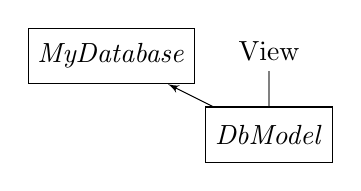
\begin{tikzpicture}[node distance=2.0cm,auto,>=latex']
            \node [int] (a) {$\mathit{MyDatabase}$};
            \node [int,below=1cm,pin={[init]above:View}] (b) [right of=a] {$\mathit{DbModel}$};
            \path[->] (b) edge node {} (a);
            \end{tikzpicture} & $\qquad \Leftrightarrow \qquad$ &
            
            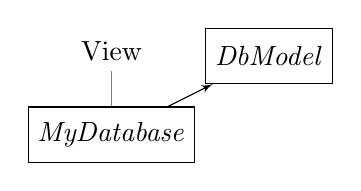
\begin{tikzpicture}[node distance=2.0cm,auto,>=latex']
            \node [int,pin={[init]above:View}] (c)  {$\mathit{MyDatabase}$};
            \node [int,above=1cm] (d) [right of=c] {$\mathit{DbModel}$};
            \path[->] (c) edge node {} (d);
            \end{tikzpicture} \\
            $\mathit{DbModel}$ object & & $\mathit{MyDatabase}$ object
        \end{tabular}
        \egroup
    \end{center}
    \caption{Cast between an $\mathit{DbModel}$ object and an $\mathit{MyDatabase}$ object} \label{fig:cast}
\end{figure}

The implementation of the illustrated cast is given below. This $\mathit{cast}$ function is part of a type class for which there are instances for every pair of sub-class and ancestor.
\begin{displaymath}
\begin{array}{lcl}
\multicolumn{3}{l}{\mathit{cast} :: \mathit{DbModelObj} \to \mathit{MyDatabaseObj}} \\
\mathit{cast}~(\mathit{DbModelEnd}~(\mathit{MyDatabaseData}~\mathit{pd})~\mathit{d}) & = & \\ \multicolumn{3}{l}{\quad \mathit{MyDatabaseStart}~\mathit{pd}~(\mathit{DbModelData}~d)} \\
\mathit{cast}~(\mathit{DbModelMiddle}~(\mathit{MyDatabaseData}~\mathit{pd})~\mathit{d}~\mathit{sub}) & = & \\ \multicolumn{3}{l}{\quad \mathit{MyDatabaseStart}~\mathit{pd}~(\mathit{DbModelStart}~d~\mathit{sub})}
\end{array}
\end{displaymath}
Casts in the other direction require a bit more work. Firstly, we need a different casting function whose result is wrapped in $\mathit{Maybe}$ to indicate that a cast from a base-class to a sub-class may not succeed. However, due to the use of existential types, we also require runtime type information about the type of the value in \emph{e.g.} the $\_\mathit{MyDatabase}\_\mathit{sub}$ field. Haskell's $\mathit{Typeable}$ type class\footnote{\url{https://hackage.haskell.org/package/base/docs/Data-Typeable.html}} may be used for this purpose.

\section{Translation}
\label{sec:auto}

Encoding object classes for our system by hand is both repetitive and error-prone. Luckily, the encoding is also well-suited for auto-generation using Template Haskell.
In this section, we propose syntactic sugar resembling the usual notation for object classes used by object-oriented languages. The corresponding encodings can automatically be generated from this syntax. Since the $\mathbf{class}$ keyword is already used for type classes in Haskell, object classes use the $\mathbf{state}$ keyword instead.
Declarations for object classes have syntax:
\begin{displaymath}
\begin{array}{l}
[\mathbf{abstract} \mid \mathbf{final}]~\mathbf{state}~\mathit{C}~\overline{\mathit{tyvar}}~[: P~\overline{\mathit{type}}]~\mathbf{where} \\
\quad \overline{\mathbf{data}~\mathit{var}~[= \mathit{expr}] :: \mathit{type}} \\
\quad \overline{[\mathbf{abstract}]~\mathit{var} :: \mathit{type}} \\
\quad \overline{\mathit{equation}}
\end{array}
\end{displaymath}
(We use the usual overline and square-bracket meta-syntax for repetition
and optional elements respectively.)
The $\mathbf{state}$ keyword is optionally preceded by either an $\mathbf{abstract}$ or $\mathbf{final}$ modifier, but cannot have both. If the $\mathbf{abstract}$ modifier is specified, the class cannot be instantiated directly, but it may include method typings marked as $\mathbf{abstract}$ which do not have an accompanying binding. Unless a class which inherits from an abstract class is abstract itself, it must implement all of its ancestors' methods which are marked as $\mathbf{abstract}$ and are therefore lacking an implementation. If a class is marked as $\mathbf{final}$, then no other class can inherit from it. This is accomplished by omitting the data constructors which allow successor $\Delta$-objects as shown in Figure \ref{tab:baseconstructors}.

The name of an object class $C$ follows the conventions for type constructors\footnote{In Haskell, this means that the name must start with an upper-case character.} and is followed by zero or more type variables. The optional $: \mathit{P}~\overline{\mathit{type}}$ component of the header of the declaration is used to specify the class's parent. $P$ must be the name of a non-final object class. There must be as many $\mathit{type}$s as there are type parameters in $P$'s definition. Any type variables used here must first be declared as type parameters of $C$.

The body of an object class declaration following the $\mathbf{where}$ keyword consists of three types of definitions which may appear in any order. A line starting with the $\mathbf{data}$ keyword is used to declare a field and must consist of at least a name and a type, but may optionally have an expression describing its default value. If no default value is specified, then it is assumed to be $\bot$. The fields in the object class declaration are desugared into fields for the state date type: 
\begin{displaymath}
\begin{array}{lcl}
\mathbf{data}~\mathit{CState}~\overline{\mathit{tyvar}} & = & \mathit{MkCState}~\{~\overline{\_\mathit{var} :: \mathit{type}}~\}
\end{array}
\end{displaymath}
The names of this data type and its single constructor can be chosen arbitrarily, since they are never exposed directly to the user. However, for consistency, we have used the name of the object class followed by $\mathit{State}$ for the name of the data type and $\mathit{Mk}$, followed by the name of the data type, for the constructor. This data type is parametrised over the same type parameters as $C$. The type alias for the state monad transformer parametrised over $\mathit{CState}$ follows:
\begin{displaymath}
\mathbf{type}~\mathit{C}~\overline{\mathit{tyvar}} = \mathit{StateT}~(\mathit{CState}~\overline{\mathit{tyvar}})~[\mathit{Identity} \mid PM~\overline{\mathit{type}}]
\end{displaymath}
By convention, the type alias is named after the object class. As with the state data type before, its type parameters are the same as in the header of the declaration for $C$. If the class has a parent, its underlying monad is that corresponding to $P$ applied to the type argument specified in the header of $C$. Otherwise, it is $\mathit{Identity}$. The last new type that results from a declaration for an object class $C$ is the data type representing objects of type $C$:
\begin{displaymath}
\mathbf{data}~\mathit{C}~\overline{\mathit{tyvar}} = \mathit{constructors}
\end{displaymath}
We refer to Figure \ref{tab:baseconstructors} for guidance on which constructors are depending on whether $C$ is a sub-class or not and which attributes it has. The $\mathit{Middle}$ constructor combines all possible fields which may be required by an object's internal state:
\begin{displaymath}
\begin{array}{l}
\forall s~d.\mathit{CLike}~s~d~(\mathit{C}~\overline{\mathit{tyvar}})~\overline{\mathit{tyvar}} \Rightarrow \mathit{CMiddle}~\{\\
\quad \begin{array}{lcl}
\_\mathit{C}\_\mathit{sup}  & :: & \mathit{PObject}~\overline{\mathit{type}}, \\
\_\mathit{C}\_\mathit{data} & :: & \mathit{CState}~\overline{\mathit{tyvar}}, \\
\_\mathit{C}\_\mathit{sub}  & :: & s~\overline{\mathit{tyvar}}
\end{array}\\
\}
\end{array}
\end{displaymath}
The existentially-quantified type variables $s$ and $d$ as well as the type class constraint are only required if the $\mathit{sub}$ field is present. $s$ refers to the object type of a sub-class and $d$ refers to the corresponding state type. The constraint enforces that the sub-class must implement all methods of $C$. The $\mathit{sup}$ field is only present in sub-classes, but never base classes. Its value is a $\Delta$-object belonging to $P$. Finally, the $\mathit{data}$ field is always present and stores the $\Delta$-object's state.

Method typings and fields are used to construct the type class representing $C$'s interface: 
\begin{displaymath}
\begin{array}{l}
\mathbf{class}~[\mathit{Monad}~m \mid \mathit{PLike}~o~s~m~\overline{\mathit{type}}] \Rightarrow \\
\quad \mathit{CLike}~o~s~m~\overline{\mathit{tyvar}} \mid o \to s, s \to o~\mathbf{where} \\
\qquad \begin{array}{l}
\_\mathit{C}\_\mathit{invoke} :: \mathit{CLike}~o'~d'~(\mathit{StateT}~(s~\overline{\mathit{tyvar}})~m)~\overline{\mathit{tyvar}} \Rightarrow \\
\qquad o'~\overline{\mathit{tyvar}} \to \\ \qquad (o'~\overline{\mathit{tyvar}} \to \mathit{StateT}~(s~\overline{\mathit{tyvar}})~m~(r,o'~\overline{\mathit{tyvar}})) \to\\\qquad
o~\overline{\mathit{tyvar}} \to m~(r,o~\overline{\mathit{tyvar}},o'~\overline{\mathit{tyvar}}) \\
\overline{\_\mathit{ext}\_\mathit{get}\_\mathit{field} :: o~\overline{\mathit{tyvar}} \to m~(\mathit{type}, o~\overline{\mathit{tyvar}}) } \\
\overline{\_\mathit{int}\_\mathit{get}\_\mathit{field} :: \mathit{StateT}~(s~\overline{\mathit{tyvar}})~m~\mathit{type}} \\
\overline{\_\mathit{ext}\_\mathit{set}\_\mathit{field} :: o~\overline{\mathit{tyvar}} \to \mathit{type} \to m~((),o~\overline{\mathit{tyvar}})} \\
\overline{\_\mathit{int}\_\mathit{set}\_\mathit{field} :: \mathit{type} \to \mathit{StateT}~(s~\overline{\mathit{tyvar}})~m~()} \\
\overline{\_\mathit{ext\_method} :: o~\overline{\mathit{tyvar}} \to \overline{\mathit{arg} \to}~m~(\mathit{result},o~\overline{\mathit{tyvar}})}\\
\overline{\_\mathit{int\_method} :: \overline{\mathit{arg} \to}~ \mathit{StateT}~(s~\overline{\mathit{tyvar}})~m~\mathit{result} }
\end{array}
\end{array}
\end{displaymath}

For each field, there is a getter and a setter. Just like methods, each has an internal and an external version. Note that we treat getters and setters as state transformers, just like methods. We take the view that they are \emph{properties} as they are found in \emph{e.g.} C\#. That is, while we have the expectation that a getter gets the value of a field and that a setter sets the value of the field, both can also potentially be implemented as arbitrary methods with matching types. Additionally, the $\_\mathit{C}\_\mathit{invoke}$ method is used by sub-classes to invoke their own methods in a monad stack set up by $C$.

An instance of this type class is generated as well as one for each type class belonging to an ancestor of $C$. Each external method's implementation pattern matches on the configuration of the object, adds a state monad transformer layer on top of the existing monad stack, and then either invokes its own, internal implementation of the method or propagates the call to a sub-class.

If $C$ is not a base class, a second instance of $\mathit{CLike}$ is generated with the underlying monad set to $\mathit{Identity}$. In this case, all methods use $\_P\_\mathit{invoke}$ on the $\Delta$-object belonging to $P$ to perform the process shown in Figure \ref{fig:invoke}:
\begin{displaymath}
\begin{array}{l}
\mathbf{instance}~\mathit{CLike}~\mathit{C}~\mathit{CState}~\mathit{Identity}~\overline{\mathit{tyvar}}~\mathbf{where}\\
\quad \begin{array}{lcl}
\mathit{method}~(\mathit{CEnd}~\mathit{sup}~\mathit{d}) & = & \mathbf{do} \\
\multicolumn{3}{l}{\quad \begin{array}{lcl}
    (r,sup',\mathit{CEnd}~\_~d') & \leftarrow & \\ 
    \multicolumn{3}{l}{ \quad \_P\_\mathit{invoke}~(\mathit{CEnd}~\mathit{sup}~d)~\mathit{method}~\mathit{sup} }\\
    \multicolumn{3}{l}{\mathit{return}~(r, \mathit{CEnd}~sup'~d')}
    \end{array}}
\end{array}
\end{array}
\end{displaymath}
%Methods are mostly standard Haskell. $<:$ and $>:$ statements are desugared into calls to the appropriate getters or setters for a field. Method invocations (identifiers containing dots) are rewritten so that the object becomes the first argument of the method and the resulting expression is then wrapped into $\mathit{runIdentity}$.

\section{Template Haskell}
\label{sec:th}

\textbf{COPIED FROM OLD VERSION}

We have implemented our system in a Haskell library\footnote{\url{https://github.com/mbg/monadic-state-hierarchies}} which primarily provides a $\mathit{QuasiQuoter}$ \citep{mainland2007s} for our object notation. Multiple state declarations may be included in a single quotation and, indeed, this is necessary if multiple state classes depend on each other. The examples in Section \ref{sec:usage} can be used exactly as shown. For example, for $\mathit{MListItem}$ we write:
\begin{displaymath}
\begin{array}{l}
[\mathit{state}\mid \mathbf{state}~\mathit{MListItem}~a~\mathbf{where} \\
\quad \begin{array}{lcl}
\mathbf{data}~\mathit{val} & :: & a \\
\mathbf{data}~\mathit{next}  & :: & \mathit{Maybe}~(\mathit{MListItem}~a)
\end{array}\\\\
\quad \begin{array}{lcl}
\mathit{insertAtEnd} & :: & \mathit{MListItem}~a \to ()\\
\mathit{insertAtEnd}~v & = & \mathbf{do} \\
\multicolumn{3}{l}{\quad \begin{array}{l}
\mathit{switch}~\mathit{next}~\$~\lambda case \\
\quad \begin{array}{lcl}
\mathit{Nothing} & \to & \mathit{next} <: \mathit{Just}~v  \\
(\mathit{Just}~n) & \to & \mathbf{do} \\
\multicolumn{3}{l}{\quad \mathit{next} <: \mathit{Just}~(\mathit{object}~(n.!\mathit{insertAtEnd})~v) }
\end{array}
\end{array}}
\end{array}\\\mid]
\end{array}
\end{displaymath}
The quotation is parsed and then translated into an abstract representation of Haskell's syntax, according to the rules shown in Section \ref{sec:auto}. Method typings must be given, similar to type classes. We parse them as standard Haskell, but their co-domains will be wrapped into \emph{e.g.} $\mathit{MListItemM}$ in the example above. Method equations are also parsed as standard Haskell, but there is no need to apply any transformations. 

In order to allow programmers to work with the object classes, our library contains a number of combinators. Most of these combinators operate on \emph{selectors} which are defined as:
\begin{displaymath}
\begin{array}{lcl}
\mathbf{data}~\mathit{Selector}~o~s~m~a~b & = & \mathit{MkMethod}~\{ \\
\multicolumn{3}{l}{\quad \begin{array}{lcl}
\mathit{mInternal} & :: & \mathit{a} \to \mathit{StateT}~s~m~b, \\
\mathit{mExternal} & :: & o \to a \to m~(b,o)
\end{array}} \\
\multicolumn{3}{l}{\} \mid \mathit{MkField}~\{} \\
\multicolumn{3}{l}{\quad \begin{array}{lcl}
\mathit{fExGet} & :: & o \to m~(b,o), \\
\mathit{fInGet} & :: & \mathit{StateT}~s~m~b, \\
\mathit{fExSet} & :: & o \to a \to m~((),o), \\
\mathit{fInSet} & :: & a \to \mathit{StateT}~s~m~b
\end{array}} \\
\multicolumn{3}{l}{\} \mid \mathit{MkCall}~\{} \\
\multicolumn{3}{l}{\quad \begin{array}{lcl}
\mathit{cCall} & :: & a \to (b,o)
\end{array}} \\
\}
\end{array}
\end{displaymath}
Intuitively, a selector is a record of all functions belonging to a field or method. The $\mathit{MkCall}$ constructor is used to represent selectors which have been applied to an object. For convenience, we define a type alias for fields since their argument and return types will always be the same:
\begin{displaymath}
\begin{array}{lcl}
\mathbf{type}~\mathit{Field}~o~s~m~a & = & \mathit{Selector}~o~s~m~a~a
\end{array}
\end{displaymath}
We enrich the type classes that are generated for object classes with selectors for all fields and methods, using the original names from the state declaration. For example, $\mathit{MListItemLike}$ contains
\begin{displaymath}
\begin{array}{l}
\mathit{val} :: \mathit{MListItemLike}~o~s~m~a \Rightarrow \\
\qquad \mathit{Field}~(o~a)~(s~a)~m~a \\
\mathit{next} ::  \mathit{MListItemLike}~o~s~m~a \Rightarrow \\
\qquad  \mathit{Field}~(o~a)~(s~a)~m~(\mathit{Maybe}~(\mathit{MListItem}~a))\\
\mathit{insertAtEnd} ::  \mathit{MListItemLike}~o~s~m~a \Rightarrow \\
\qquad  \mathit{Selector}~(o~a)~(s~a)~m~(\mathit{MListItem}~a)~()\\
\end{array}
\end{displaymath}
in addition to the type class methods shown in Section \ref{sec:auto}. This allows us to use the field and method names directly in any context without any compile-time transformations which resolve them to the appropriate functions. For example, in the instance for $\mathit{MListItem}$, $\mathit{next}$ has the following value:
\begin{displaymath}
\mathit{next} = \mathit{MkField} \mathit{\_get\_next} \mathit{\_get\_next}' \mathit{\_set\_next} \mathit{\_set\_next}'
\end{displaymath}
When used in \emph{e.g.} the $<:$ operator, the appropriate setter is extracted from the record and applied to the new value for the field:
\begin{displaymath}
\begin{array}{l}
(<:)  ::  \mathit{Monad}~m \Rightarrow \mathit{Field}~o~s~m~\mathit{val} \to \mathit{val} \to \mathit{StateT}~s~m~()\\
(\mathit{MkField}~\_~\_~\_~s') <: val  =  s val
\end{array}
\end{displaymath}
Objects and selectors can be combined using the $.!$ operator which in turn constructs a new selector which can then be used by one of the combinators. The $.!$ is part of the $\mathit{Object}$ type class which in our implementation is the super class of all objects, instead of $\mathit{Monad}$, although $\mathit{Monad}$ is still the superclass of $\mathit{Object}$:
\begin{displaymath}
\begin{array}{l}
\mathbf{class}~\mathit{Monad}~m \Rightarrow \mathit{Object}~\mathit{obj}~m~\mathbf{where}\\
\quad (.!) :: \mathit{obj} \to \mathit{Selector}~\mathit{obj}~s~m~\mathit{arg}~\mathit{ret} \to \\ \qquad \mathit{Selector}~\mathit{obj}~s~m~\mathit{arg}~\mathit{ret}
\end{array}
\end{displaymath}
There is one instance of this class for all base object classes:
\begin{displaymath}
\begin{array}{l}
\mathbf{instance}~\mathit{Object}~a~\mathit{Identity}~\mathbf{where}\\
\quad \begin{array}{lcl}
\mathit{obj}~.!~(\mathit{MkMethod}~\mathit{int}~\mathit{ext}) & = & \\
\multicolumn{3}{l}{\quad \mathit{MkCall}~ \$~\lambda \mathit{arg} \to \mathit{runIdentity}~\$~\mathit{ext}~\mathit{obj}~\mathit{arg} } %\\
%\mathit{obj}~.!~(\mathit{MkField}~g~\_~s~\_) & = & \\
% \multicolumn{3}{l}{\quad \mathit{MkCall}~\$~\mathit{const}~\$~\mathit{runIdentity}~\$ ~g~\mathit{obj}}
\end{array}
\end{array}
\end{displaymath}
For example, if an object is combined with a selector, then we create a wrapper function around the method after applying it to the object. $\mathit{MkCall}$ values are then used by \emph{e.g.} the $\mathit{object}$ and $\mathit{result}$ combinators as follows:
\begin{displaymath}
\begin{array}{l}
\mathit{object} :: \mathit{Selector}~o~s~\mathit{Identity}~\mathit{arg}~\mathit{ret} \to arg \to o\\
\mathit{object}~(\mathit{MkCall}~\mathit{call})  = \mathit{snd} \circ \mathit{call}
\end{array}
\end{displaymath}




\section{Related work}
\label{sec:related}

Extending Haskell with an object system is not a new idea. Previous work evaluated various approaches to constructing object systems within Haskell and emphasised encoding information about object classes in the type system~\cite{kiselyov2005haskell}, which our encoding does not. Their library supports many of the principal features of object-oriented languages, but uses IO references to accomplish this while we wish to remain pure. There has also been work to allow Haskell to interact with object-oriented languages more easily, such as a language extension allowing object-oriented-style overloading in Haskell~\cite{shields2001object}. Type classes are also used to establish a subtyping relation. However, their work does not allow object-oriented style code to be written in Haskell itself.

The popular \texttt{lens} library by Edward Kmett\footnote{\url{https://hackage.haskell.org/package/lens}} and similar other libraries provide types and combinators for the traversal and manipulation of data structures. A $\mathit{Lens}$ combines a getter and setter for a field, similarly to our selectors. Lenses can also be composed to traverse nested data structures.
Combining lenses with our encoding of objects in future work
would enable the vast number of combinators in the \texttt{lens} library to be used on top of our system.

While most programming languages with object-oriented features are impure, theoretical backing for our system comes from formalisations of pure object calculi based on the $\lambda$-calculus~\citet{pierce1994simple}. Methods in this system are state transformers like in ours, taking objects as arguments and returning updated objects. We believe that the explicitness of a purely-functional object system allows for more flexibility than the implicitness of an impure system.

%In more theoretical work,~\cite{Pierce93simpletype-theoretic} present A typed $\lambda$-calculus with support for encapsulation, message passing, subtyping, and inheritance is presented by. Methods in this calculus are state transformers, but they do not form stacks of state monad transformers. Instead, methods simply use the object as state as in traditional object-oriented programming.

The expression problem is concerned with the choice between different ways in which programs may be extended with new functionality without having to change any of the existing code. A classical example of this is wishing to extend a programming language with new features without having to change any existing code. Our example in Section \ref{sec:encoding} demonstrates how this can partially be approached in our system. We have also drawn an analogy between the expression problem and the ``monad transformer problem''. 

Other approaches to modular data types exist for Haskell as well. Open data types and functions is a proposed extension for Haskell which enables data types and functions to be marked as ``open''. A data type marked with this keyword allows new constructors and function equations to be added after the initial declaration. This is accomplished by generating normal data types and functions from all open declarations within a program. While this approach has the advantage that it does not introduce any fundamentally new concepts to the language, it does require whole-program compilation and changes the order in which pattern matching occurs~\cite{loh2006open}.

Modular data types can be constructed in Haskell without any new extensions to the type system using the \emph{data types \`a la carte technique}~\cite{swierstra2008data}. Unlike open data types, it does not require whole-program compilation, but instead it requires a stronger grasp of the underlying techniques. To the authors' knowledge, there is no simple notation for the \`a la carte technique. This technique has been used to construct \emph{e.g.} modular compilers in which independent language fragments can introduce effects to the overall language~\cite{day2012towards}. It is not clear how easily effects can be interleaved in our system, since we assume a fixed ordering of effects.

%One alternative to the monad transformer library called \emph{Monatron}~\cite{jaskelioff2011monatron} which features an improved lifting mechanism at the cost of increased implementation complexity improves upon the \texttt{mtl} library, but shifts the difficulty from library users to library authors. \emph{Monad zippers} and \emph{monad views}~\cite{schrijvers2011monads} which are used to hide and address parts of monad stacks respectively provide another interesting approach to dealing with the complexity of monad transformers.

%One of the most promising solutions so far has been presented in~\cite{kiselyov2013extensible} where a single monad, parametrised over a set of effect handlers~\cite{plotkin2009handlers} is used to implement an effect system in Haskell. The order of effects is not fixed on the type-level, but is determined on the value level. This system is also more efficient than monad transformers since it only needs to find a matching handler when a given effect is required. Monad transformers, on the other hand, always execute all of their effects between computations, even if most of them are not required.

\section{Conclusions and future work}
\label{sec:conclusions}

We have shown how several concepts in object-oriented programming related to concepts in functional programming. Most notably, we have established a link between monad transformers and inheritance. In order to take advantage of this connection, we have encoded an object system based on state monad transformers in pure Haskell. Our encoding also has a notation of coercive subtyping which allows for the construction of modular data types in Haskell. Additionally, we have described a process for translating to our encoding from a simple object-oriented language. This process is implemented in a Haskell library, enabling programmers to use object classes in their Haskell programs without having to resort to a different language or impurity. 

The type classes which support the inheritance mechanism hide calls to the $\mathit{lift}$ function of monad transformers from the programmer, while also allowing more fine-grained control through the opportunity for method overriding. Each layer of our monad stack is mapped to a corresponding object class. We believe that this is a powerful representation of monad transformers which we plan to explore further in future work to allow for non-state classes.

A major limitation of our encoding compared to popular object-oriented languages is the lack of aliasing. While we do not believe that aliasing is an essential feature of an object system, it is often considered a key feature of object-oriented programming. Unfortunately, it requires references to an object to be shareable so that an update through one can be observed through the others -- a side effect. In impure languages, this is accomplished by storing all objects in a global heap, but this makes reasoning about such programs difficult. A good compromise may be the introduction of localised heaps which are shared between all functions which possess an alias to the same object. This may be accomplished with the help of the $\mathit{ST}$ monad \cite{launchbury1995state} which provides local, mutable state in Haskell. Such a system would not only improve our encoding, but matches similar efforts in object-oriented languages to better encapsulate objects -- see, for example, the essay by Hogg\cite{hogg1992geneva} on controlling object aliasing or ownership types\cite{clarke1998ownership}.

Outside of the context of Haskell, it may also be interesting to design a language with an object system for effect in mind. This could lead to a simpler representation of objects through corresponding language support, potentially leading to greater computational efficiency. However, we have not yet investigated how our encoding performs. 



\section{Motivation}
\label{sec:usage}

\textbf{THIS NEEDS TO BE MERGED INTO THE OTHER CHAPTERS}

Before diving into the mechanics of our encoding, let us consider some examples of what can be done with it in the notation which we introduce in detail in Section \ref{sec:auto}. % with object-oriented concepts in a functional setting before introducing [it] in detail in Section \ref{sec:auto}

As a simple example, we begin with an implementation of OO-style linked lists, for which we require two object classes. First, we define a class of list items containing values of some type $a$. Such state class declarations consist of three components: 
\begin{enumerate}
    \item A head containing the name, parameters and, optionally, parent of the class.
    \item Field declarations describing the state of instances of the class.
    \item Methods: functions with implicit access to an instance of the class.
\end{enumerate}
The below declaration introduces a new object class $\mathit{MListItem}$ with two fields, $\mathit{val}$ and $\mathit{next}$, as well as one method named $\mathit{insertAtEnd}$. To insert items at the end of an OO-style linked list, we need to traverse the list to find the last element.  $\mathit{insertAtEnd}$ implements this behaviour by inspecting the value of the $\mathit{next}$ field. If its current value is $\mathit{Nothing}$, then it is set to the $\mathit{MListItem}$ object that was provided as argument to the method. Otherwise, it calls $\mathit{insertAtEnd}$ on the current value of $\mathit{next}$.
\begin{displaymath}
\begin{array}{l}
\mathbf{state}~\mathit{MListItem}~a~\mathbf{where} \\
\quad \begin{array}{lcl}
\mathbf{data}~\mathit{val} & :: & a \\
\mathbf{data}~\mathit{next}  & :: & \mathit{Maybe}~(\mathit{MListItem}~a)
\end{array}\\\\
\quad \begin{array}{lcl}
\mathit{insertAtEnd} & :: & \mathit{MListItem}~a \to ()\\
\mathit{insertAtEnd}~v & = & \mathbf{do} \\
\multicolumn{3}{l}{\quad \begin{array}{l}
    \mathit{switch}~\mathit{next}~\$~\lambda case \\
    \quad \begin{array}{lcl}
        \mathit{Nothing} & \to & \mathit{next} <: \mathit{Just}~v  \\
        (\mathit{Just}~n) & \to & \mathbf{do} \\
            \multicolumn{3}{l}{\quad \mathit{next} <: \mathit{Just}~(\mathit{object}~(n.!\mathit{insertAtEnd})~v) }
    \end{array}
    \end{array}}
\end{array}
\end{array}
\end{displaymath}
Note that the explicit typing for $\mathit{insertAtEnd}$ gives it a pure type, despite having the effect of transforming an object's state. The reason for this design choice is twofold. Firstly, the effectful type can be inferred from the scope in which the method is defined, similarly to the way that class constraints are added implicitly to the methods belonging to a type class. Secondly, the corresponding monad is not given a name until we desugar the class definition, therefore programmers would have to refer to a name that does not occur anywhere in their code. However, if the name that is generated for the monad is predictable, then there is no fundamental reason why the effect cannot be made explicit.

Methods themselves are just regular Haskell functions which make use of combinators provided by our library. The $\mathit{selector} <: \mathit{value}$ operator sets the value of a field indicated by $\mathit{selector}$ to $\mathit{value}$. Field and method names serve as selectors and may be combined using the $.!$ operator. 

Selectors for fields simultaneously refer to both getters and setters. We therefore need to provide them with enough context to determine whether we wish to use the getter or setter. For instance, the $\mathit{switch}$ combinator applied to the $\mathit{next}$ selector in the example below obtains the value of $\mathit{next}$ using the corresponding getter and then passes it on to the second argument. We describe selectors fully in Section \ref{sec:th}.

When methods, such as $\mathit{insertAtEnd}$, are invoked, they always return a pair consisting of a result and an updated object. Since object-oriented languages are generally impure, they can simply mutate an object in-place. In a purely functional setting, we can only do this if the object is contained within the state of a state monad. Therefore, in general, the programmer has to decide whether they want the updated object, the result, or both. We provide combinators, such as $\mathit{object}$ and $\mathit{result}$, to invoke methods identified by a selector and to return either the updated object or the result of the method, respectively.

For convenience, we define a smart constructor\footnote{A user-defined function used to construct new values of some type} for new objects of type $\mathit{MListItem}$ below. The $\mathbf{new}$ function, applied to initial values for the corresponding fields, is used to instantiate an object class. Unlike in most object-oriented languages where the name of the class we wish to instantiate needs to be specified, we rely on Haskell's type inference to do this for us. Note that the explicit typing is not required:
\begin{displaymath}
\begin{array}{lcl}
\mathit{mkItem} & :: & a \to \mathit{MListItem}~a \\
\mathit{mkItem}~v & = & \mathit{new}~v~\mathit{Nothing}
\end{array}
\end{displaymath}
By setting the $\mathit{next}$ field of a $\mathit{MListItem}$ object to a value other than $\mathit{Nothing}$, elements can be added to the list. A value of $\mathit{Nothing}$ indicates the end of the list. To account for the empty list, we declare a $\mathit{MList}$ class which we use as the start of a linked list:
\begin{displaymath}
\begin{array}{l}
\mathbf{state}~\mathit{MList}~a~\mathbf{where} \\
\quad \begin{array}{lcl}
\mathbf{data}~\mathit{root}  & :: & \mathit{Maybe}~(\mathit{MListItem}~a)
\end{array}\\\\
\quad \begin{array}{lcl}
\mathit{insert} & :: & a \to () \\
%\mathit{insert}~v & = & \mathbf{do} \\
%\multicolumn{3}{l}{\quad \begin{array}{lcl}
%\multicolumn{3}{l}{\mathbf{let}}\\
%\multicolumn{3}{l}{\quad \mathit{item} = \mathit{mkItem}~v} \\
%\mathit{mr} & <: & \mathit{root} \\
%\multicolumn{3}{l}{\mathbf{case}~\mathit{mr}~\mathbf{of}} \\
%\multicolumn{3}{l}{\quad \begin{array}{lcl}
%\mathit{Nothing} & \to & \mathbf{do}~\mathit{Just}~\mathit{item} >: \mathit{root} \\
%(\mathit{Just}~r) & \to & \mathbf{do}~\mathit{Just}~(\mathit{snd}~\$~r.\mathit{insertTo}~\mathit{item}) >: \mathit{root}
%\end{array}}
%\end{array}}
\mathit{toList} & :: & [a]
\end{array}
\end{array}
\end{displaymath}
We omit the definitions of the $\mathit{insert}$ and $\mathit{toList}$ methods as they follow similar structures as the $\mathit{insertTo}$ method of the $\mathit{MListItem}$ class. The $\mathit{mkItem}$ function can be used to turn the value to insert into a $\mathit{MListItem}$ object. To test our construction, we define a function that, given an OO-style list of integers, inserts a few integers, and finally converts it to a functional list:
\begin{displaymath}
\begin{array}{lcl}
\mathit{test} & :: & \mathit{MList}~\mathit{Int} \to [\mathit{Int}]\\
\mathit{test}~l & = & \mathbf{let} \\
\multicolumn{3}{l}{\quad \begin{array}{lcl}
    a & = & \mathit{object}~(l.!\mathit{insert}~23)\\
    b & = & \mathit{object}~(a.!\mathit{insert}~16)\\
    c & = & \mathit{object}~(b.!\mathit{insert}~42)\\
    d & = & \mathit{object}~(c.!\mathit{insert}~24)\\
    \end{array}}\\
\multicolumn{3}{l}{\mathbf{in}~\mathit{result}~(d.!\mathit{toList})~()}
\end{array}
\end{displaymath}
Applying $\mathit{test}$ to an empty list results in the following reduction:
\begin{displaymath}
\begin{array}{cl}
& \mathit{test}~(\mathit{new}~\mathit{Nothing}) \\
\Rightarrow & [23,16,42,24]
\end{array}
\end{displaymath}
Now suppose that we wish to define a class of lists which are always sorted according to some predicate. Instead of starting from scratch, we define a class $\mathit{SList}$ which derives from $\mathit{MList}$. This is indicated using a notation for inheritance borrowed from C++:

\begin{displaymath}
\begin{array}{l}
\mathbf{state}~\mathit{SList}~a : \mathit{MList}~a~\mathbf{where} \\
\quad \begin{array}{lcl}
\mathbf{data}~\mathit{pred}  & :: & a \to a \to \mathit{Bool}
\end{array}\\\\
\quad \begin{array}{lcl}
\mathit{insert} & :: & a \to ()\\
\mathit{insert}~v & = & \mathbf{do} \\
\multicolumn{3}{l}{\quad \begin{array}{lcl}
    \multicolumn{3}{l}{\mathbf{let}}\\
    \multicolumn{3}{l}{\quad \mathit{item} = \mathit{mkItem}~v} \\
    \multicolumn{3}{l}{\mathit{switch}~\mathit{root}~\$~\lambda \mathbf{case}} \\
    \multicolumn{3}{l}{\quad \begin{array}{lcl}
        \mathit{Nothing} & \to & \mathit{root} <: \mathit{Just}~\mathit{item}  \\
        (\mathit{Just}~r) & \to & \mathbf{do} \\
        \multicolumn{3}{l}{\quad \begin{array}{lcl}
            p & \leftarrow & \mathit{value}~\mathit{pred} \\
            \mathit{root} & <: & \mathit{Just}~(\mathit{helper}~v~p~r) 
            \end{array}}
        \end{array}}
    \end{array}}
\end{array}
\end{array}
\end{displaymath}
By deriving $\mathit{SList}$ from $\mathit{MList}$, it has inherited all fields and methods of its parent. Additionally, we have added a $\mathit{pred}$ field used to store the predicate according to which the list should be sorted. We have also overriden the definition of $\mathit{insert}$ to use a $\mathit{helper}$ function which inserts a new item at the correct position within the list, according to $\mathit{pred}$. The definition of $\mathit{helper}$ is given below. Note that this function does not need to be a member of $\mathit{SList}$.
\begin{displaymath}
\begin{array}{lcl}
\mathit{helper} & :: &  a \to (a \to a \to \mathit{Bool}) \to \\
& & \mathit{MListItem}~a \to \mathit{MListItem}~a \\
\mathit{helper}~v~p~i & = & \mathbf{let} \\
\multicolumn{3}{l}{\quad \begin{array}{lcl}
    \mathit{rv} & = & \mathit{value}~(i.!\mathit{val}) \\
    \mathit{item} & = & \mathit{mkItem}~v
    \end{array}}\\
\multicolumn{3}{l}{\quad \mathbf{in}~\mathbf{if}~p~v~rv~\mathbf{then}~\mathbf{case}~\mathit{value}~(c.!\mathit{next})~\mathbf{of}} \\
\multicolumn{3}{l}{\quad \quad \begin{array}{lcl}
    \mathit{Nothing} & \to & i.\mathit{setNext}~\$~\mathit{Just}~\mathit{item} \\
    (\mathit{Just}~n) & \to & i.\mathit{setNext}~\$~\mathit{Just}~\$~\mathit{helper}~v~p~n 
    \end{array}} \\
\multicolumn{3}{l}{\quad \mathbf{else}~\mathit{item}.\mathit{setNext}~(\mathit{Just}~c)}
\end{array}
\end{displaymath}
Applying the $\mathit{test}$ function we defined earlier to an $\mathit{SList}$ object directly is not possible. In other words, even though we consider $\mathit{SList}$ to be a sub-type of $\mathit{MList}$, an explicit cast must be inserted in the form of a $\mathit{downcast}$ function:
\begin{displaymath}
\begin{array}{cl}
& \mathit{test}~(\mathit{downcast}~(\mathbf{new}~(\mathit{Nothing},(>)))) \\
\Rightarrow & [16,23,24,42]
\end{array}
\end{displaymath}   
Evaluating this expression results in a sorted list. This example shows how, using a familiar notation, a program can first be constructed and then extended without having to modify any of the initial code. In addition, we have a convenient means of working with the effect of mutable state.

A more useful example is the implementation of the abstract representation and denotational semantics of a simple expression language:
\begin{displaymath}
\begin{array}{lcl}
\multicolumn{3}{l}{e = n \in \mathbb{N} \mid e+e} \\\\

\denote{\cdot} & : & e \to \mathbb{N}\\
\denote{n} & = & n \\
\denote{e_0+e_1} & = & \denote{e_0} + \denote{e_1}
\end{array}
\end{displaymath}
In functional languages, the abstract representation of the grammar would normally be defined using an algebraic data type with two constructors, one for each production. In object-oriented languages, the representation consists of an abstract base class with a sub-class for each production. Figure \ref{fig:razor} shows how to write this in our notation.
\begin{figure}
\begin{displaymath}
\begin{array}{l}
\mathbf{abstract}~\mathbf{state}~\mathit{Expr}~\mathbf{where} \\
\quad \begin{array}{lcl}
\mathbf{abstract}~\mathit{eval} & :: & \mathit{Int}
\end{array} \\\\
\mathbf{state}~\mathit{Val} : \mathit{Expr}~\mathbf{where} \\
\quad \begin{array}{lcl}
\multicolumn{3}{l}{\mathbf{data}~\mathit{val} = 0  :: \mathit{Int}} \\\\
\mathit{eval} & :: & \mathit{Int} \\
\mathit{eval} & = & \mathit{value}~\mathit{val}
\end{array} \\\\
\mathbf{state}~\mathit{Add} : \mathit{Expr}~\mathbf{where} \\
\quad \begin{array}{lcl}
\multicolumn{3}{l}{\mathbf{data}~\mathit{left}  :: \mathit{Expr}} \\
\multicolumn{3}{l}{\mathbf{data}~\mathit{right}  :: \mathit{Expr}} \\\\
\mathit{eval} & :: & \mathit{Int} \\
\mathit{eval} & = & \mathbf{do} \\
\multicolumn{3}{l}{\quad \begin{array}{lcl}
    l & \leftarrow & \mathit{result}~(left.!eval)~() \\
    r & \leftarrow & \mathit{result}~(right.!eval)~() \\
    \multicolumn{3}{l}{\mathit{return}~(l + r)}
    \end{array}} 
\end{array} 
\end{array}
\end{displaymath}
\caption{Expression language}
\label{fig:razor}
\end{figure}

We can now construct arbitrary expressions consisting of addition and values with the help of the $\mathit{new}$ function mentioned previously.

If we wish to extend this language with \emph{e.g.} a multiplication operator, then we would normally have to extend the corresponding algebraic data type with an additional constructor and we would also have to add a new case to the evaluation function. This may not be desirable if, for example, both are located in a library. In our system, we can simply add a new object class which inherits from $\mathit{Expr}$ to extend the language and do not have to change any of the existing code:
\begin{displaymath}
\begin{array}{l}
\mathbf{state}~\mathit{Mul} : \mathit{Expr}~\mathbf{where} \\
\quad \begin{array}{lcl}
\multicolumn{3}{l}{\mathbf{data}~\mathit{left}  :: \mathit{Expr}} \\
\multicolumn{3}{l}{\mathbf{data}~\mathit{right}  :: \mathit{Expr}} \\\\
\mathit{eval} & :: & \mathit{Int} \\
\mathit{eval} & = & \mathbf{do} \\
\multicolumn{3}{l}{\quad \begin{array}{lcl}
    l & \leftarrow & \mathit{result}~(left.!eval)~() \\
    r & \leftarrow & \mathit{result}~(right.!eval)~() \\
    \multicolumn{3}{l}{\mathit{return}~(l \times r)}
    \end{array}} 
\end{array}
\end{array}
\end{displaymath}
Importantly, $\mathit{Mul}$ objects can be used as arguments for \emph{e.g.} $\mathit{Add}$ objects, even though we did't know about $\mathit{Mul}$ when we declared the $\mathit{Add}$ class.


\subsubsection*{Acknowledgments.} We would like to thank the anonymous referees and Dominic Orchard for their valuable feedback on an earlier versions of this paper. This work was supported by EPSRC.

%TODO: these need to be embedded and properly formatted for the springer format
\bibliographystyle{abbrv}
\bibliography{pwmsh}

\end{document}
